\Subsection{Билет 9: ! Несобственные интегралы от неотрицательных функций. Признак сравнения. Следствия.}

\begin{theorem} \thmslashn

    $f \ge 0 \;\; f \in C[a,b)$

    Тогда сходимость $\int\limits_a^b f(x) \, dx$ равносильна ограниченности сверху первообразной F.

\end{theorem}

\begin{proof} \thmslashn

    $F(y) := \int\limits_{a}^{y} f$

    $\int\limits_a^b f(x) \, dx =\lim\limits_{c \to b-} F(c) - F(a)$, $F(a) = 0$ (из утверждения выше)

    $F(z) = F(y) + \int\limits_{y}^{z} f \ge F(y)$, где $\int\limits_{y}^{z} f \ge 0$ при $y < z$ $\implies F(y)$ монотонно возрастает.

    Итого, $F(y)$ имеет предел и монотонно возрастает. Для монотонно возрастающих функция существование предела равносильно ограниченности сверху

\end{proof}

\begin{consequence} \thmslashn

    $f,g \in C[a,b)  \;\; 0 \le f \le g $
    \begin{enumerate}
    
        \item Если $\int\limits_{a}^{b} g$ сходится, то $\int\limits_{a}^{b} f$ сходится.
        
        \item Если $\int\limits_{a}^{b} f$ расходится, то $\int\limits_{a}^{b} g$ расходится.
        
    \end{enumerate}

\end{consequence}

\begin{proof} \thmslashn

    $G(y) := \int\limits_{a}^{y} g, \;\; F(y) := \int\limits_{a}^{y} f \implies F \le G$  
    \begin{enumerate}
    
        \item $\int\limits_{a}^{b} g$ сходится $\implies$ G ограничена сверху $\implies$ F ограничена сверху $\implies \int\limits_{a}^{b} f$ сходится.
        
        \item От противного. Пусть $\int\limits_{a}^{b} g$ сходится, тогда и $\int\limits_{a}^{b} f$ сходится по первому пункту. Противоречие.
        
    \end{enumerate}

\end{proof}

\begin{remark}

    \begin{enumerate}
    
        \item Неравенству $f \le g$ достаточно выполнения для аргументов, близких к b.

        \begin{proof} \thmslashn

            $\int\limits_{a}^{b} f = \int\limits_{a}^{c} f + \int\limits_{c}^{b} f$
    
            Для второго слагаемого $f \le g$, используем следствие.
        \end{proof}
    
        \item Вместо $f \le g$ можно использовать и $f = O(g)$

        \begin{proof} \thmslashn

            $\int\limits_{a}^{b} Cg = C \int\limits_{a}^{b} g $ -- сходится.

        \end{proof}
    
        \item Если $f \ge 0$, $f \in C[a,+\infty)$ и $f = O(\frac1{x^{1+\eps}})$ при $\eps > 0$, то $\int\limits_{a}^{+\infty} f $ сходится.

        \begin{proof} \thmslashn

            $f \in O(\frac1{x^{1+\eps}}) \implies f \le M\cdot \frac1{x^{1+\eps}} =: g$
			
			Надо доказать, что $\int\limits_a^{+\infty} g$ сходится.
			
			$\int\limits_a^{+\infty}  M\cdot \frac1{x^{1+\eps}} = M\int\limits_a^{+\infty} \frac1{x^{1+\eps}}$ -- сходится.

        \end{proof}

    \end{enumerate}

\end{remark}

\begin{consequence} \thmslashn

    $f, g \ge 0 \;\; f,g \in C[a,b)$ и $f \sim g$ при $x \to b-$
		
    Тогда $\int\limits_a^b f$ и $\int\limits_a^b g$ ведут себя одинаково.

\end{consequence}

\begin{proof} \thmslashn

    $f \sim g \implies$ найдется такое $c$, что $\frac{g}{2} \le f \le 2g$ при $x > c$

    Если $\int\limits_{a}^{b} g $ сходится, то $f \le 2g \implies \int\limits_{a}^{b} f$ сходится.

    Если $\int\limits_{a}^{b} f $ сходится, то $g \le 2f \implies \int\limits_{a}^{b} g$ сходится.

\end{proof}

\begin{remark} \thmslashn

    $f \ge 0 \;\; f \in C[a,+\infty)$ и $\int_a^{+\infty} f$ сходится.

    Это НЕ значит $f(x) \to 0$ при $x \to +\infty$

\end{remark}

Дана функция, изображенная на графике (спасибо за это Герману). Площади треугольников убывают: $S_1 = \frac{1}{2}$, $S_2 = \frac{1}{4}$, $S_3 = \frac{1}{8}$, $\ldots$, $S_n = \frac{1}{2}\cdot 2\cdot 2^{-n} = \frac{1}{2^n}$
  \begin{center}
    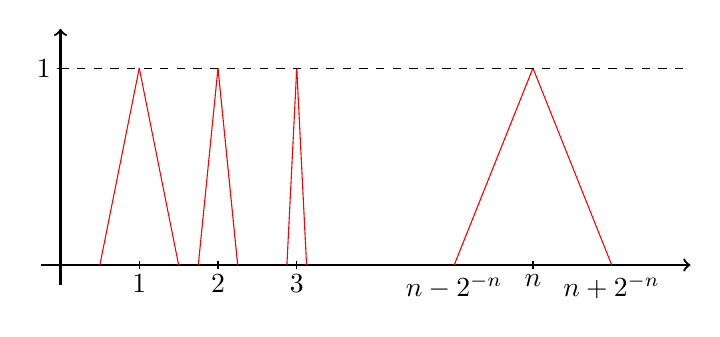
\begin{tikzpicture}[]
    
      \draw[thick, ->] (-0.25, 0) -> (8, 0);
      \draw[thick, ->] (0, -0.25) -> (0, 3);
      
      \draw[-] (1,-0.05) -- (1,0.05);
      \node[below] at (1, 0) {$1$};
    
      \draw[-] (2,-0.05) -- (2,0.05);
      \node[below] at (2, 0) {$2$};
      
      \draw[-] (3,-0.05) -- (3,0.05);
      \node[below] at (3, 0) {$3$};
      
      \draw[-] (6,-0.05) -- (6,0.05);
      \node[below] at (6, 0) {$n$};
      
      \draw[-] (-0.05,2.5) -- (0.05,2.5);
      \node[left] at (0, 2.5) {$1$};
      
      \draw[red, -] (0.5, 0) -- (1, 2.5);
      \draw[red, -] (1.5, 0) -- (1, 2.5);
      
      \draw[red, -] (1.75, 0) -- (2, 2.5);
      \draw[red, -] (2.25, 0) -- (2, 2.5);
      
      \draw[red, -] (2.875, 0) -- (3, 2.5);
      \draw[red, -] (3.125, 0) -- (3, 2.5);
      
      \draw[red, -] (5, 0) -- (6, 2.5);
      \draw[red, -] (7, 0) -- (6, 2.5);
      
      \node[below] at (5, 0) {$n - 2^{-n}$};
      
      \node[below] at (7, 0) {$n + 2^{-n}$};
      
      \draw[dashed] (0, 2.5) -- (8, 2.5);
      
    \end{tikzpicture}
  \end{center}
